\documentclass[11pt]{article}
\usepackage[pdftex]{graphicx}
\usepackage[utf8]{inputenc}
\usepackage{float}										% positioning of floats such as graphics, tables
\usepackage{subfig}
\usepackage{amsmath}									% advanced math extensions
\usepackage{latexsym}									% other mathematical symbols
\usepackage{amssymb}									% other mathematical symbols
\usepackage{amsthm}										% theorem environment
\usepackage{commath}									% differential operators \dif
\usepackage{mathrsfs}									% mathscr font in math mode																
\usepackage{setspace}									% modifiable line pitch
\usepackage{array}										% extends possibility of LaTeX to handle tables
\usepackage{hyperref}									% best package wo je h�ts gits
\usepackage{parskip}									% no indention for new paragraphs
\usepackage{framed}										% framed environment for framed text
\usepackage{fancyhdr} 									% change header and footer of any page of the document
\usepackage{mdwlist}									% smaller line pitch for \itemize, \enumerate
\usepackage{color}										% adds support for colored text
\usepackage[english]{babel}
\usepackage{tikz}										% nice drawing environment
\usetikzlibrary{arrows}
\usetikzlibrary{positioning}

\renewcommand{\labelitemi}{--}
\newcommand{\unit}[1]{\ensuremath{\, \mathrm{#1}}}			% units

\definecolor{darkblue}{rgb}{0,0,.4}
\definecolor{darkgreen}{rgb}{0,0.5,0}
\hypersetup{pdfborder={0 0 0},colorlinks=true,linkcolor=darkblue,citecolor=darkgreen}


\newcommand{\lint}{\mathlarger{\int}}
\newcommand{\R}{\mathbb{R}}
\newcommand{\C}{\mathbb{C}}
\newcommand{\N}{\mathbb{N}}
\newcommand{\Z}{\mathbb{Z}}
\newcommand{\Q}{\mathbb{Q}}
\newcommand{\linspan}{\operatorname{span}}
\newcommand{\nextpar}{\vspace{5pt}}
\newcommand{\type}{~\mathtt}

\newcommand{\HRule}{\rule{\linewidth}{0.5mm}}
\usepackage[a4paper,left=2.5cm, right=2.5 cm, top=2.5cm, bottom=2cm]{geometry}


\usepackage{pdfpages}

\pagestyle{fancy}
\fancyhead{}
\fancyfoot{} 
\fancyhead[L]{\sffamily  {\small FastCode}}
\fancyhead[R]{\sffamily  {\small Homework 3}}


\begin{document}
\hspace{0.2 in}
\begin{center}
	\begin{Large}
		\textbf{Homework 3: Solutions Dominik Gresch}
	\end{Large}
\end{center}
\subsection*{Exercise 1: Cache mechanics}
	\begin{itemize}
		\item[a)] The general solution is given by
		\begin{align*} 
		 M = \frac{1}{2(b s + t)}&\Bigg( s + \lceil t/b \rceil + \sum\limits_{j=0}^{\lceil t / b\rceil - 1} \Theta \left(\sum\limits_{i=(j+1)b-1}^{bs + t - 1} \delta_{\beta_i, s+j} \right)  \\ & + 
		\sum\limits_{j=0}^{\lceil t / b\rceil - 1} \Theta \left(\sum\limits_{i=\min[b(s+j+1)-1, b s + t -1 ]}^{2bs + t - 1} \delta_{\beta_i, j} \right)  + \sum\limits_{j=0}^{\lceil t/b \rceil - 1} \delta_{\alpha_i,\beta_{i-1}}\cdot\left(1-\delta_{\gamma_i,0}\right) \Bigg)
		\end{align*}
		where 

		\[ \Theta(x) = \left\{
			\begin{array}{ll}
				0~~  & \text{if } x \leq 0 \\
				1 & \text{else}
			\end{array} \right.  \]
		\begin{align*}
			\alpha_i =& \lfloor (bs + ((bi)\%(bs + t)))/b \rfloor\%2s\\
			\beta_i =& \lfloor ((bi)\%(bs + t))/b \rfloor\%2s\\
			\gamma_i =& (i\%(bs + t))\%2s
		\end{align*}
		
		and $\delta$ is the Kronecker Delta. $\alpha_i$ and $\beta_i$ describe in which set \texttt{y} and \texttt{x} are at iteration \texttt{i}, $\delta_i$ the block offset of \texttt{y}.\par The first 2 terms come from the misses that happen because \texttt{y} gets loaded into cache the first time.\par The third term comes from cacheblocks at the beginning of \texttt{y} that have been evicted between the time when \texttt{y} first accessed them and the time \texttt{y} accesses them again (second part of the loop).\par The fourth term is the same, but with the end of \texttt{y} that overlaps with \texttt{x} (in terms of cache address).\par Finally, the last term describes cache misses due to a ``race condition'', between \texttt{x} and \texttt{y}, those are misses where \texttt{x} and \texttt{y} are at the same cache location at the same time (but not when \texttt{y} accesses the first element of a block, because those are already accounted for).\par
		I have provided a \texttt{Mathematica} file for evaluation: see \texttt{/ex01/ex01.nb}\\
		As a last remark, for \texttt{(s,b,t)} which fulfil the condition $\mathtt{t\leq b\leq s}$ or $\mathtt{b + t \leq s}$ (I only tested these limits numerically), this term becomes much easier:
		\[ M = \frac{s + \lceil t/b\rceil  }{2(bs + t)} \]
		
		\item[b)] \texttt{x}: for the first 7 \texttt{i}, there are only misses (access the first element of a cache block each time). After that, there will be 6 hits (accessing the second element). For $\mathtt{i \in \{13, 25\}}$, there will be misses only for the elements that have been evicted due to conflicts with \texttt{y} (i.e. \texttt{i = 13, 19})
		\[ \Rightarrow \mathtt{x: MMMMMMMHHHHHH~MHHHHHMHHHHHH} \]
		\texttt{y}: For the first 13 \texttt{i}, there are alternating misses and hits. After that, there will be a miss only for \texttt{i = 13} and \texttt{i = 25} (the elements that have been evicted due to conflict with \texttt{x}).
		\[ \Rightarrow \mathtt{y: MHMHMHMHMHMHM~MHHHHHHHHHHM} \]
		\item[c)] Since \texttt{sum} is in a register, the traffic will be exactly $2 \type{doubles} \cdot \type{\# misses}$. There are 18 \texttt{misses}, hence 
		\[ Q = 18 \cdot 2 \cdot 8 \type{bytes} = 288 \type{bytes} \]
		There are 2 \texttt{flops} in each loop iteration, 26 iteration steps 
		\[ \Rightarrow W = 52 \type{flops} \Rightarrow I = \frac{13}{72}\type{\frac{flop}{byte}} \]
	\end{itemize}
	\newpage
\subsection*{Exercise 2: Cache mechanics}
	\begin{itemize}
		\item[a)] The upper bound for \texttt{I} is determined by the minimum number of bytes read (reading the three variables exactly once) and the number of flops.
		\begin{align*}
			Q& \geq (12 + 4 + 3) \type{doubles} = 152 \type{bytes}\\
			W& = 12 \type{add} + 12 \type{mult} = 24 \type{flop}\\
			\Rightarrow I& \leq \frac{12}{76} \type{\frac{flop}{byte}}
		\end{align*}
		\item[b)] In every iteration of the innermost loop, there is fist an access to \texttt{A[i][j]} and \texttt{x[j]} and then an access to \texttt{y[i]} (the multiplication gets evaluated first).\par Each cache block fits exactly one \texttt{double}.\par
		Looking only at \texttt{A} and \texttt{x}, each even \texttt{j} fills up the \texttt{0} - th set and each odd \texttt{j} fills up the \texttt{1}st set. Since \texttt{A} does not use the same value twice and \texttt{x} only uses the same value after 4 \texttt{j} (when all previous values have already been evicted), there are no cache hits for either \texttt{A} or \texttt{x}. This results in 12 misses for \texttt{A} and 12 misses for \texttt{x}.\par
		For \texttt{y}, there are two different scenarios. If \texttt{i \% 2 == 0} (i.e. \texttt{y[i]} is in the first set), the hit/miss pattern for \texttt{j = 0,...,3} is \texttt{MHMH} (2 misses). If \texttt{i \% 2 == 1} (i.e. \texttt{y[i]} is in the second set), the miss/hit pattern is \texttt{MMHM} (3 misses). Because the first scenario happens twice and the second once, this gives 7 misses for \texttt{y}.\par
		\[ M_{L_1} = \frac{12 + 12 + 7}{36}\type{\frac{misses}{acces}} = \frac{31}{36}\type{\frac{misses}{access}} \]
		\item[c)] Every read miss creates $8 \type{bytes}$ of traffic. Additionally, \texttt{y} has to be written to memory exactly the same number of times as misses for \texttt{y} (each time the value gets brought in it will eventually have to be written back).\par
		\[ Q = (31 + 7) \cdot 8 \type{bytes} = 304 \type{bytes} \]
		of traffic, and hence
		\[ I_{L_1} = \frac{3}{38} \type{\frac{flop}{byte}} \]
		\item[d)] The variables all fit into the $L_2$ - cache (no conflicts): \texttt{A} takes up one block per set for the first 6 sets, \texttt{x} and \texttt{y} fit into the two blocks of the 7-th and 8-th set respectively. \\
		The only misses come from bringing the variables in once. Since each block contains 2 \texttt{doubles}, this gives rise to 
		\begin{itemize}
			\item $\frac{12}{2} \type{misses} = 6 \type{misses}$ for \texttt{A}
			\item $\frac{4}{2} \type{misses} = 2 \type{misses}$ for \texttt{x}
			\item $\lceil\frac{3}{2}\rceil \type{misses} = 2 \type{misses}$ for \texttt{y}
		\end{itemize}
		\[ \Rightarrow 10 \type{misses} \Rightarrow M_{L_2} = \frac{10}{3\cdot 12} \type{\frac{misses}{access}} = \frac{5}{18}\type{\frac{misses}{access}} \]
		\item[e)] Memory traffic comes from reading each variable and writing \texttt{y}. For \texttt{y}, there is an additional \texttt{double} of memory traffic since it doesn't fit perfectly into the second block (effectively, 4 \texttt{double} of traffic for each complete read / write of \texttt{y}).
		\[ \Rightarrow Q = (12 + 4 + 4\cdot 2) \cdot 8 \type{byte} = 192 \type{byte} \Rightarrow I_{L_2} = \frac{1}{8}\type{\frac{flop}{byte}} \]
	\end{itemize}

\subsection*{Exercise 3: Associativity}
	I do not agree with your statement. Counterexample: \par 
	Let $\mathtt{x}$, $\mathtt{y}$ and $\mathtt{z}$ be 3 arrays of size $\mathtt{B / 8}$ (they fit exactly into one block), and their addresses such that (for the direct mapped cache), $\mathtt{x}$ gets mapped into the $\mathtt{0}$ - th set, $\mathtt{y}$ and $\mathtt{z}$ into the $\mathtt{S / 2}$ - th. Of course, for the 2 - way associative cache, they will all be mapped into the $\mathtt{0}$-th cache set.\\
	Now consider the following code (assuming \texttt{sum} is in registers, otherwise cold cache):
	\begin{tabbing} 
		\=\texttt{double sum = 0;}\\
		\>\texttt{for(int i = 0; i < B / 8; ++i) \{ }\\
		\>\hspace*{1cm} \= \texttt{sum += x[i];}\\
		\> \> \texttt{sum += y[i];}\\
		\> \> \texttt{sum += z[i];}\\
		\> \texttt{\}}
	\end{tabbing}
	
	Whilst the direct mapped cache produces hits for \texttt{x} (after the initial miss), and misses only for \texttt{y} and \texttt{z}, the 2 - way associative cache produces only misses.\\
	direct mapped: \texttt{MMMHMMHMM...}\\
	2 - way associative: \texttt{MMMMMMMMM...}\\
	The reason for this is that \texttt{x} stays in cache in the direct mapped case whilst it gets evicted (because it is least recently used) in the 2 - way associative case.
	\begin{figure}[H]\centering
		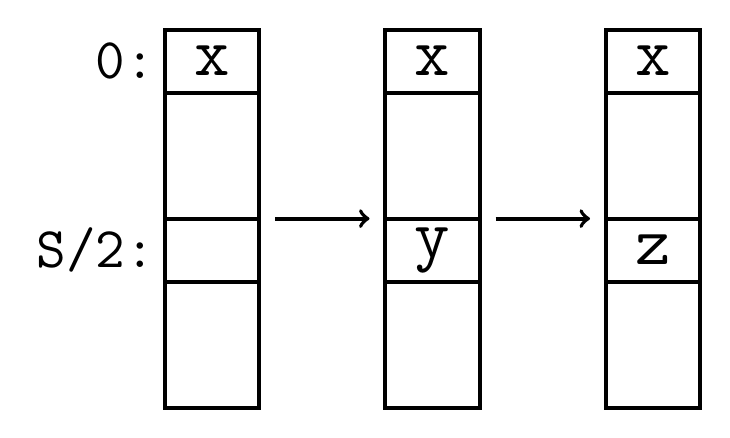
\begin{tikzpicture}[scale = 0.4]
			%\draw[help lines] (0,0) grid (20,10);
			\draw[line width = 0.05cm] (1, 10) rectangle (4, 8);
			\draw[line width = 0.05cm] (1, 8) rectangle (4, 4);
			\draw[line width = 0.05cm] (1, 4) rectangle (4, 2);
			\draw[line width = 0.05cm] (1, 2) rectangle (4, -2);
			\node at (2.5, 9) {\Huge{\texttt{x}}};
			\node[left] at (1, 9) {\huge{\texttt{0:}}};
			\node[left] at (1, 3) {\huge{\texttt{S/2:}}};
			
			\draw[->, line width = 0.05cm] (4.5 ,4) -- (7.5, 4);
			
			\draw[line width = 0.05cm] (8, 10) rectangle (11, 8);
			\draw[line width = 0.05cm] (8, 8) rectangle (11, 4);
			\draw[line width = 0.05cm] (8, 4) rectangle (11, 2);
			\draw[line width = 0.05cm] (8, 2) rectangle (11, -2);
			\node at (9.5, 9) {\Huge{\texttt{x}}};
			\node at (9.5, 3) {\Huge{\texttt{y}}};
			
			\draw[->, line width = 0.05cm] (11.5 ,4) -- (14.5, 4);
			
			\draw[line width = 0.05cm] (15, 10) rectangle (18, 8);
			\draw[line width = 0.05cm] (15, 8) rectangle (18, 4);
			\draw[line width = 0.05cm] (15, 4) rectangle (18, 2);
			\draw[line width = 0.05cm] (15, 2) rectangle (18, -2);
			\node at (16.5, 9) {\Huge{\texttt{x}}};
			\node at (16.5, 3) {\Huge{\texttt{z}}};
		\end{tikzpicture}
		\caption{first loop iteration with direct mapped cache}
	\end{figure}
	\begin{figure}[H]\centering
		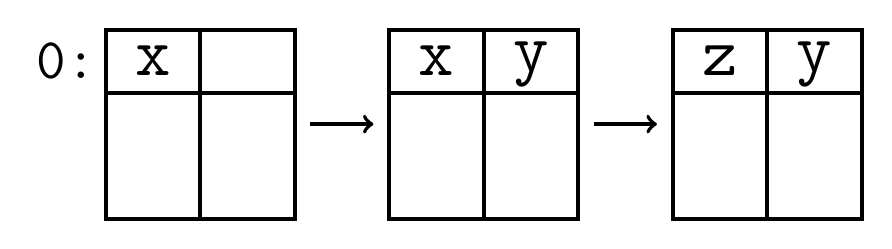
\begin{tikzpicture}[scale = 0.4]
			%\draw[help lines] (0,0) grid (20,10);
			\draw[line width = 0.05cm] (1, 10) rectangle (4, 8);
			\draw[line width = 0.05cm] (1, 8) rectangle (4, 4);
			\draw[line width = 0.05cm] (4, 10) rectangle (7, 8);
			\draw[line width = 0.05cm] (4, 8) rectangle (7, 4);
			\node at (2.5, 9) {\Huge{\texttt{x}}};
			\node[left] at (1, 9) {\huge{\texttt{0:}}};
			
			\draw[->, line width = 0.05cm] (7.5, 7) -- (9.5, 7);
			
			\draw[line width = 0.05cm] (10, 10) rectangle (13, 8);
			\draw[line width = 0.05cm] (10, 8) rectangle (13, 4);
			\draw[line width = 0.05cm] (13, 10) rectangle (16, 8);
			\draw[line width = 0.05cm] (13, 8) rectangle (16, 4);
			\node at (11.5, 9) {\Huge{\texttt{x}}};
			\node at (14.5, 8.9) {\Huge{\texttt{y}}};
			
			\draw[->, line width = 0.05cm] (16.5, 7) -- (18.5, 7);
			
			\draw[line width = 0.05cm] (19, 10) rectangle (22, 8);
			\draw[line width = 0.05cm] (19, 8) rectangle (22, 4);
			\draw[line width = 0.05cm] (22, 10) rectangle (25, 8);
			\draw[line width = 0.05cm] (22, 8) rectangle (25, 4);
			\node at (20.5, 9) {\Huge{\texttt{z}}};
			\node at (23.5, 8.9) {\Huge{\texttt{y}}};
			
			
		\end{tikzpicture}
		\caption{first loop iteration with 2 - way associative cache}
	\end{figure}
		
	
\end{document}